% Copyright (c) 2015-2018, AIT Austrian Institute of Technology GmbH.
% REM All rights reserved. See file POWERFACTORY_FMU_LICENSE.txt for details.

\chapter{Installation and Configuration}

\section{Software requirements}

The \fmipp \pf FMU Export Utility is intended to run on Windows~10. The following applications need to be installed prior to installing the \fmipp \pf FMU Export Utility:
\begin{itemize}
  \item \href{http://www.digsilent.com/}{DIgSILENT~\pfversion}, including the additional package \emph{External C interface for dynamic models}
  \item \href{https://www.python.org/}{\python}: only required when creating FMUs from the command line (tested with \python~3.7)
  \item \href{https://www.visualstudio.com/vs/older-downloads/}{Microsoft Visual Studio Community 2017}: only required for generating FMUs according to FMI version 1.0
\end{itemize}

\subsubsection*{Note:}
The current version of the \fmipp \pf FMU Export Utility has been specifically compiled to work with \pfversion.
It will very likely fail to run with older versions, newer version might work.


\section{Installation}
\label{sec:install}

\subsection*{Step~1: Download and extract}

To install the \fmipp \pf FMU Export Utility , proceed as follows:
\begin{itemize}
  \item Download the latest version as ZIP-file from the \href{http://sourceforge.net/projects/powerfactory-fmu/files/latest/download}{download page}.
  \item Unzip the installation file into any sub directory (referred to as the \emph{installation directory}).
\end{itemize}

\subsection*{Step~2: Running the installation script}

\subsubsection*{Installation via the graphical user interface}

Switch to the installation directory and start program \texttt{powerfactory\_fmu\_install.exe} (double-click).
This should bring up the window shown in Figure~\ref{fig:gui_install}.
Provide the path to the \pf installation directory and press \textit{Start}.

\begin{figure}[h!]
%\vspace*{1em}
\centering{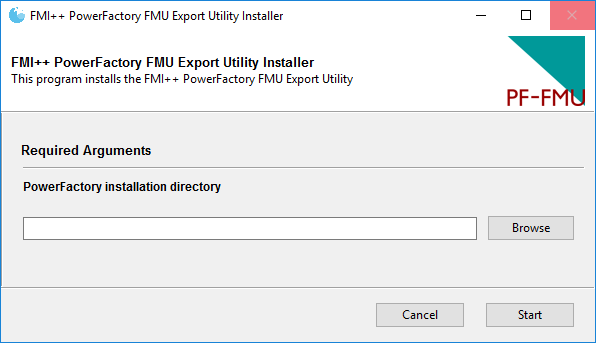
\includegraphics[width=0.9\textwidth]{gui_install}}
\vspace*{-2mm}
\caption{Graphical user interface for installing the \fmipp \pf FMU Export Utility.}
\label{fig:gui_install}
\end{figure}


\subsubsection*{Installation via the command line}

Alternatively, installation can be done from the command prompt window by executing a \python script.
Please refer to the \href{https://docs.python.org/3/faq/windows.html}{\python~FAQ} in case you need assistance with this.

Open the command prompt window, change to the installation directory and execute the script \texttt{powerfactory\_fmu\_install.py}:
\begin{verbatim}
python.exe powerfactory_fmu_install.py <pf_install_dir>
\end{verbatim}
where \texttt{<pf\_install\_dir>} is the path to your local \pf installation directory (for instance \texttt{C:\symbol{92}DIgSILENT\symbol{92}pf2019}).

After successful installation, the \pf installation directory contains one new file called \texttt{fmiadapter.dll}. This is the DLL implementation of the compiled DSL model used for interacting with \pf in RMS simulations (see Section~\ref{\label{sec:export:create_model_rms}).


\subsection*{Step~3: Updating the Windows system path}

Finally, the \pf installation directory has to be added to the Windows system path. For instruction on how to do that please refer for instance \href{https://de.mathworks.com/matlabcentral/answers/94933-how-do-i-set-my-system-path-under-windows}{here}.
